\documentclass[final]{svjour2}
\usepackage{amsmath}
\usepackage{graphicx}
\usepackage{rotating}
\usepackage{amssymb}
\usepackage{mathptmx}
\usepackage[numbers]{natbib}
\usepackage{float}
\usepackage[section]{placeins}
\usepackage{tabularx}
\usepackage{booktabs}
\usepackage{color}
\makeatletter
\journalname{Journal of Low Temperature Physics}
%%%%%%%%%%%%%%%%%%%%%%%%%%%%%% Textclass specific LaTeX commands.
%%%%%%%%%%%%%%%%%%%%%%%%%%%%%% User specified LaTeX commands.
\bibpunct{}{}{,}{s}{}{,}

\begin{document}

\newcommand{\hdblarrow}{H\makebox[0.9ex][l]{$\downdownarrows$}-}
\title{Material Selection for Cryogenic Support Structures}

\author{E. Kramer \and N. Kellaris  \and M. Daal  \and B. Sadoulet \and S. Golwala \and M. Hollister}

\institute{Department of Physics, U.C. Berkeley,\\ Berkeley, CA 94709, USA\\
\email{ekramer@berkeley.edu}}

\date{07.29.2013}

\maketitle

\begin{abstract}

Design specifications for the support structures of low temperature instrumentation often call for low thermal conductivity between temperature stages, high stiffness, and specific load bearing capabilities.  While overall geometric design plays an important role in both overall strength and heat conduction between stages, material selection can affect a structure's properties significantly.  In this contribution, we suggest and compare several alternative materials to the current standard materials for building cryogenic support structures.

\keywords{Cryogenic Tower, Thermal Conductivity, Material Strength}
 
\end{abstract}

\section{Introduction} 
Cryogenic support structures are typically engineered to meet three design specifications: low thermal conductance, high strength, and high stiffness. Creating support structures that obtain the lowest thermal conductance between temperature stages while still remaining structurally adequate to support forces imposed during operation at base temperature and during handling at room temperature is an design optimization problem. The thermal consideration usually results in structures suspended by elements possessing minimized cross-sectional area -- thin plates, webs of yarn, slender rods or tubes. The application will dictate which of strength or stiffness that imposes next most limiting design constraint. Focusing on the case of stiffness, we draw attention to the fact that both stiffness and power conducted proportional to the cross-sectional area, $A$, divided by the length, $l$, of the structure support members.\cite{Hastings1993} As we shall explain, this provides a helpful parameterization for the selection of cryogenic support structural materials.  

\section{Material Selection Design Parameters}

The property that describes the stiffness or elasticity of a material is its Young's modulus\footnote{Young's modulus is formally defined for tensile stresses, but one can easily extend the notion to compressive forces on a material. Young's Modulus is sometimes called \em{elastic modulus} or \em{modulus of elasticity}.}. It is slope of the stress versus strain curve and is sometimes different for tensile stress (the `tensile modulus') and the compressive stress (the `compressive modulus'). It should also be pointed out that different samples of the same material may have different moduli as a result of their defect characteristics, heat treatments, etc. When loading a cryogenic support structure, the forces experienced generally tend to be of the same magnitude in both compressive and tensile directions.  Because of this, the smaller of the two moduli, the tensile modulus or the compressive modulus, must be focused on in order to keep a sufficient factor of safety and prevent premature failure.

It is also important to note the other properties of the material being used.  Ductile materials, such as most metals, tend to fail from shear forces first, while brittle materials like carbon fibers fail from normal forces first.  Another aspect of material selection is that of metallic versus non-metallic support. Metallic supports can be quite stiff, however they are not ideal for structures with electrically isolated stages.  The shape of the thermal conductivity cure also plays an important roll as steep thermal conductivity curves creates susceptability to thermal run-aways in the cryostat. 

Overall when deciding on materials, they must be stiff enough to not fail under expected loads ranges while keeping their cross section is low as possible to minimize the amount of heat transfer between temperature stages. Because stiffness and power conducted are both proportional to the cross-sectional area divided by the length, $A/l$, we can normalize the Young's modulus of a material by its thermal conductivity in order to compare multiple materials for use in these structures. Runyan\cite{Runyan2008} et al. presented a very similar plot comparing different materials not featured in this contribution.  In general because a high stiffness and low thermal conductance is typically desired, when choosing materials we desire the smallest Thermal conductivity to Young's Modulus ratio.\cite{Hastings1993}  A variety of materials exist with acceptable strength and thermal properties for use in a cryogenic support structure setting.  In the plot below we present a few newer useful materials along with familiar standbys that have the desired low thermal conductivity to Young's Modulus ratio.

\begin{figure}[!ht]
\begin{center}
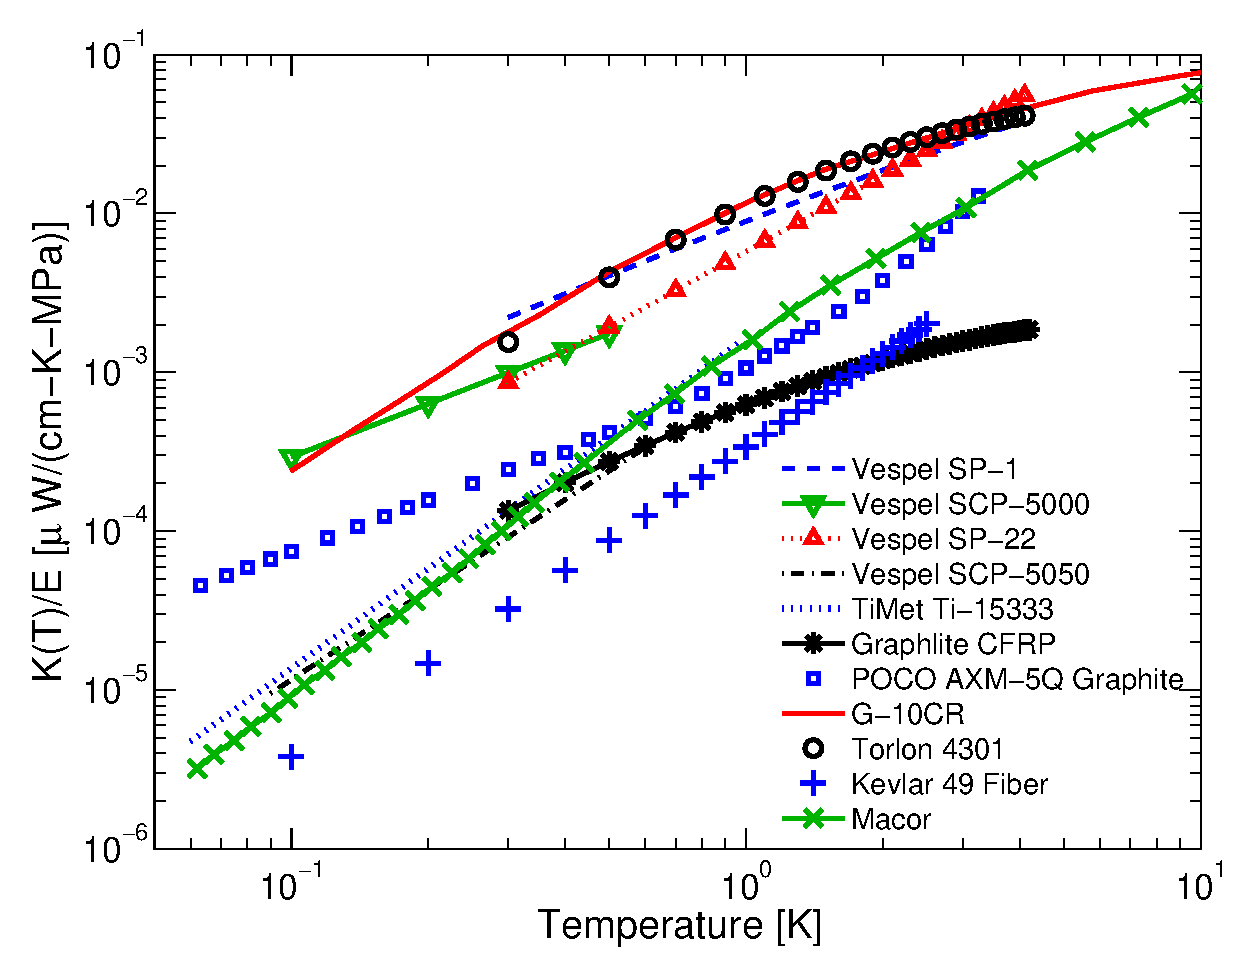
\includegraphics[%
  width=1.0\linewidth,
  keepaspectratio]{Mats}
\end{center}
\caption{A selection of useful materials with their room temperature Young's modulus normalized by their thermal conductivity.  Lower values are desirable as support materials. \color{red}{Need to call out which data came from publication. Also, need to add stainless steel!} \cite{Doty1981}\cite{Kasen1981}\cite{Runyan2008}\cite{Kellaris2013}\cite{Woodcraft2009}\cite{Woodcraft2009_2}\cite{Ventura2009} }
\label{Mats}
\end{figure}

\begin{figure}[!ht]
\begin{center}
\includegraphics[%
  width=0.75\linewidth,
  keepaspectratio]{Table}
\end{center}
\caption{Some material strength and thermal properties of some select materials at room temperature.}
\label{SW}
\end{figure}

\section{Conclusions}
While many different geometric design solutions [once the geometric design of a cryogenic support as been selected, the materials used to build it, determine its strength, stiffness and thermal conductance. A parameter useful in material selection is the material's thermal conductivity normalized to its Young's Modulus.  Unlike design geometry alterations, a change of material used to build a structure tends to be a much easier and predictable way to improve upon a design in terms of its performance under a force or heat load. Also changes in material of a structure have the advantage of avoiding the necessity to make changes in the governing equations or model for theoretical evaluation due to the fact that material properties tend to be well defined dependent variables in both. For geometric designs that already exist and cannot be altered, a judicious change of support material using the data presented here could improve performance without necessarily entailing further detailed modeling.

\begin{acknowledgements}
We would like to thank Sanjay Govindjee for technical assistance. We acknowledge support and funding from the Department of Energy and the National Science Foundation.
\end{acknowledgements}

\begin{thebibliography}{99}

%%%%%%%%% Structure bibliography items %%%%%%%%%%
%%%%%%%%%%%%%%%%%%%%%%%%%%%%%%%%%%%%%%%%%%%%%%%%%
\bibitem{Hastings1993}
Peter R. Hastings and D.M. Montgomery. {\it Support of cooled components in astronomical instruments. Cryogenics} \textbf{2633(11):1032–1036}, 1993.

%%%%%% Young's modulus bibliography items %%%%%%%%%
%%%%%%%%%%%%%%%%%%%%%%%%%%%%%%%%%%%%%%%%%%%%%%%%%%%

\bibitem{Doty1981}
F.D. Doty and P.D. Ellis, {\it Rev. Sci. Instrum.} \textbf{52(12)}, 1868, (1981).

\bibitem{Kasen1981}
M.B. Kasen, G.R. MacDonald, D.H. Beekman, Jr., and R.E. Schramm, {\it Advances in Cryogenic Engineering Materials} \textbf{26}, 235, (1981). 

%%%% Thermal conductivity bibliography items %%%%
%%%%%%%%%%%%%%%%%%%%%%%%%%%%%%%%%%%%%%%%%%%%%%%%%

%%% Vespel SP-1, Vespel SP-22, Graphlite CFRP, Torlon 4301
\bibitem{Runyan2008}
M.C. Runyan and W.C. Jones, {\it Cryogenics} \textbf{48}, 448, (2008).

%%% Vespel SCP-5000, Vespel SCP-5050, Ti 15-3-3-3
\bibitem{Kellaris2013}
N.A. Kellaris. {\it Unpublished thermal conductivity measurements}, (2013).

%%% AXM-5Q
\bibitem{Woodcraft2009}
A.L. Woodcraft, M. Barucci, P.R. Hastings, L. Lolli, V. Martelli, L. Risegari, and G. Ventura, {\it Cryogenics} \textbf{49}, 159, (2009).

%%% G-10CR & Macor
\bibitem{Woodcraft2009_2}
A.L. Woodcraft and A. Gray, {\it Low Temp. Detectors 13, Proceedings of the 13$^{th}$ International Workshop}, \textbf{1185}, 681, (2009).

%%% Kevlar 49
\bibitem{Ventura2009}
G. Ventura and V. Martelli, {\it Cryogenics} \textbf{49}, 376, (2009).

\end{thebibliography}

\end{document}
